\subsection{Technologies in physical layer}

In this section, several physical layer technologies which may be used in our system are picked and explained. The four technologies picked are: 
\begin{itemize}[noitemsep]
    \item Bluetooth
    \item 802.11
    \item ZigBee
    \item Z-wave
\end{itemize}

\paragraph{Bluetooth}
The first technology to look into is \textit{Bluetooth}. Bluetooth is a standard which specifies wireless transmissions of data. It is designed to be used for data exchange between mostly portable devices such as smart-phones, input devices (keyboard, etc.), headsets, etc. It uses free 2.4~GHz ISM-band, so it prone to interference with other radio technologies using this frequency band (such as Wi-Fi). Therefore, adaptive frequency hopping was implemented. The Bluetooth frequency band is divided into 79 hop carriers (1~MHz difference). During its operation, devices switch between frequencies repeatedly - 1600~times a second, with schedule determined by the master device. It was designed for point to point communication, but piconets can be created with a master device and up to 7 slaves. Bluetooth is designed for use in \acrfull{pan} and therefore it is not the best solution for \acrshort{iot} systems. All devices in the piconet switch the hop carriers simultaneously and every piconet has its own jumping order defined upon creation.

However, the main feature of Bluetooth is arguably its frequency hopping scheme. The Bluetooth frequency band is divided into 79 hop carriers. During its operation, devices switch between frequencies repeatedly, with schedule determined by the master device. All devices in the piconet switch the hop carriers simultaneously and every piconet has its own jumping order defined upon creation.
% 
\paragraph{802.11}
There are many versions of IEEE 802.11 which have properties that differs in terms of range, maximum speed, power efficiency, frequency band used or intended application. Recently, however, a new 802.11 was published\footnotemark: 802.11ah or \textit{Wi-Fi HaLow}, which is designed to be used in IoT or low powered and low data rate networks.
\footnotetext{\url{http://www.ieee802.org/11/Reports/802.11_Timelines.htm\#tgah}, accessed 13-05-2018}
% 
On the other hand, it has a long range of up to 1 km which is almost double of today’s Wi-Fi~\cite{EricZeman2016WiFiInformationWeek}. Reason for that is the use of 900~MHz frequency band, as the lower frequency bands allow bigger range and easier penetration through obstacles but slower data rates, which is not a problem in WSNs. Its maximum data rate is 40~Mbits/s which much less compared to other 802.11 standards which maximum data rates are measured in Gbits/s~\cite{Jean-JacquesDeLisle2015Whats802.11ah}. At the moment, this technology is not spread much, because it is new. It supports up to 8000 nodes connected to a single access point as well as creation of mesh networks, which increases even further increases number of nodes and range~\cite{ClausHetting2017GiantHaLow}.
% 
\paragraph{ZigBee}
ZigBee is a wireless standard which has been developed specifically for use in WSNs. Its maximum throughput is 250kbit/s and usual range is 10-100~meters (but can be up to 500~meters). However, if a mesh networking is used, it may reach much further. ZigBee was designed to be less expensive to implement in devices, need low power so devices can run even years on a battery, less complex and to have lower data rate as sensor nodes usually do not need to send lots of data.
% 
It also uses 128-bit key for symmetric \acrshort{aes} encryption~\cite{PaulLamkin2018Z-WaveHome}. These are reasons why it is well suited for use in WSNs and deployment in smart homes, industrial automation, smart badges, etc. It uses 2.4~GHz unlicensed band for transmission. There may be maximum 65~536~nodes in the same network\footnotemark. ZigBee defines physical as well as \acrshort{mac} layer~\cite{Sohraby2007WirelessApplications}.
\footnotetext{{\url{http://www.telecomabc.com/z/zigbee.html}, accessed 13-05-2018}}
% 
\paragraph{Z-Wave}
Z-wave can be considered as a competitor to Zigbee. It was developed for use in WSNs as well and it uses licensed 900~MHz frequency for communication. That means it does not suffer from interference that much. It is much more energy efficient than Wi-Fi, nodes can run on battery several years (even 10 years in borderline cases~\cite{PaulLamkin2018Z-WaveHome}) and the range is bigger than the Bluetooth’s one, up to 100 meters in point to point connection but nodes can form full mesh network and reach much further. Downside of Z-wave is its maximum number of nodes in a network -- 232, which makes it not ideal for use in industrial scenarios~\cite{PaulLamkin2018Z-WaveHome}. It is safe and it runs 128-bit \acrshort{aes} encryption, same as ZigBee\footnotemark. Its maximum data rate speed is 40~kbits/s which less than ZigBee’s speed but sufficient for IoT use. 
\footnotetext{\url{https://www.sigmadesigns.com/news/mandatory-security-implementation-for-all-z-wave-certified-iot-devices-takes-effect-today/}, accessed 13-05-2018}
% 
\paragraph{Conclusion}
In a container scenario, all of above mentioned technologies may be used because they range, throughput and maximum number of nodes are sufficient, even power efficiency is similar though it is probably a factor that has a biggest weight in this scenario. Unfortunately, the exact power consumption was not measured, but as most of these technologies were designed specifically for use in WSNs, they are all efficient. Our suggestion however, is to use Z-wave as it is using sub 1~GHz frequency which provides higher power saving.
For a container to hub scenario, Z-wave is not suitable as it can have only 232 nodes connected to one access point which is not sufficient. Bluetooth was designed mainly for use in \acrshort{pan} network with up to 7 slaves and a master node in one piconet which is not sufficient as well (even though scatternet may be composed from several piconets). Regarding ZigBee and Wi-Fi HaLow, both of them are suitable for our use as in both technologies thousands of nodes may be connected to a single sink, data rate is sufficient in both of them and as sending nodes are connected to a power source, power efficiency is not a deal. If one of then should be chosen however, Wi-Fi HaLow would be suggested because of higher possible data rates and bigger range.

% There exist many wireless protocols like IEEE 802.15.4 – ZigBee, IEEE 802.15.1 – Bluetooth, IEEE 802.16 – WiMax or IEEE 802.11a/b/g/n – wireless Lan. Each one of them is suitable for use in different scenario, has different characteristics and may span more than one layer. ZigBee devices are designed for low power consumption, small range and data throughput, which makes them ideal for use in difficult to reach locations where it can run on battery for years. Bluetooth is typically used on devices like smartphones, laptops but also sensors which can run on batter for several days, while being able to achieve higher throughput and short-range communication. On the other hand, 802.11 provides the highest range and throughput but also power consumption, ideal for use in devices being plugged in. Summarising table may be seen in Figure~\ref{fig:protocol-comparison} and more in-depth comparison will follow in later chapter.

% \begin{figure}
%     \centering
%     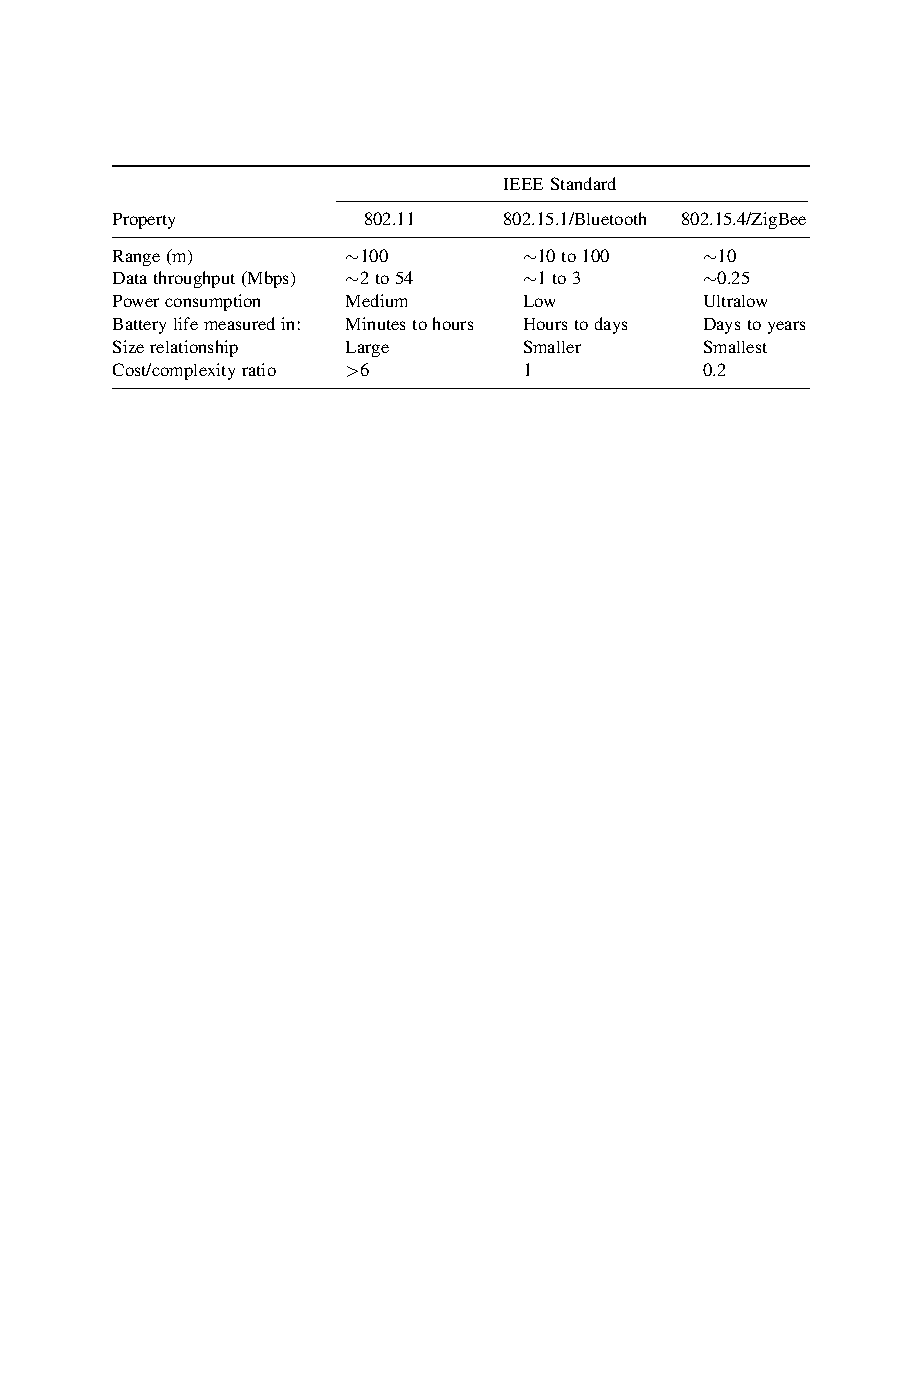
\includegraphics[width=0.8\textwidth]{00images/protocol-comparison}
%     \caption{Comparison of IEEE standards for selected physical layer protocols. Taken from~\cite{Sohraby2007WirelessApplications}.}
%     \label{fig:protocol-comparison}
% \end{figure}